\documentclass[aspectratio=169,10pt]{beamer}

% ==============================================================================
% Configuración de Tema y Colores
% ==============================================================================
\usetheme{Boadilla}
\usecolortheme{whale}

% Paleta institucional moderna y limpia
\definecolor{DarkBlue}{HTML}{0F172A}
\definecolor{AccentBlue}{HTML}{1E40AF}
\definecolor{SoftBlue}{HTML}{3B82F6}
\definecolor{LightBg}{HTML}{F8FAFC}
\definecolor{CardBg}{HTML}{F1F5F9}
\definecolor{TextDark}{HTML}{0F172A}

\setbeamercolor{palette primary}{bg=DarkBlue,fg=white}
\setbeamercolor{palette secondary}{bg=AccentBlue,fg=white}
\setbeamercolor{palette tertiary}{bg=SoftBlue,fg=white}
\setbeamercolor{structure}{fg=AccentBlue}
\setbeamercolor{frametitle}{bg=DarkBlue,fg=white}
\setbeamercolor{title}{bg=DarkBlue,fg=white}
\setbeamercolor{block title}{bg=AccentBlue,fg=white}
\setbeamercolor{block body}{bg=CardBg,fg=TextDark}

% Opciones tipográficas y paquetes
\usepackage[utf8]{inputenc}
\usepackage[spanish]{babel}
\usepackage{amsmath,amssymb}
\usepackage{graphicx}
\usepackage{booktabs}
\usepackage{microtype}
\usepackage{helvet}
\usepackage{tikz}
\usetikzlibrary{shapes.geometric, arrows.meta, positioning, calc}

% Colores de las etapas del pipeline
\definecolor{Stage1}{HTML}{1E40AF}
\definecolor{Stage2}{HTML}{0D9488}
\definecolor{Stage3}{HTML}{D97706}
\definecolor{Stage4}{HTML}{7C3AED}

% Desactivar barra de navegación inferior innecesaria
\setbeamertemplate{navigation symbols}{}
\setbeamertemplate{footline}[frame number]

% Título y Metadatos
\title[Avances Ñandú sEMG]{Avances en el proyecto de decodificación de las vocales}
\subtitle{Hardware, Sensores Musculares y Modelado}
\author[S. Prado Rodríguez]{Santiago Prado Rodríguez}
\institute[LSD - UBA]{Laboratorio de Sistemas Dinámicos (LSD) \\ Departamento de Física, FCEyN - Universidad de Buenos Aires}
\date{Octubre 2026}

\begin{document}

% ------------------------------------------------------------------------------
% Slide 1: Portada
% ------------------------------------------------------------------------------
\begin{frame}[plain]
    \titlepage
\end{frame}

% ------------------------------------------------------------------------------
% Slide: Índice de contenidos
% ------------------------------------------------------------------------------
\begin{frame}{Índice de contenidos \hfill \textnormal{\footnotesize Octubre 2026}}
    \begin{columns}[c]
        \begin{column}{0.85\textwidth}
            \tableofcontents
        \end{column}
    \end{columns}
\end{frame}

% ==============================================================================
% SECCIÓN: Hardware e Instrumentación
% ==============================================================================
\section{Hardware e Instrumentación}

% ------------------------------------------------------------------------------
% Slide 2: Hardware y Blindaje: Reducción del Ruido Eléctrico
% ------------------------------------------------------------------------------
\begin{frame}{Blindaje de cables: eliminando el zumbido de 50 Hz \hfill \textnormal{\footnotesize 14/10/2026}}
    \begin{columns}[c]
        \begin{column}{0.48\textwidth}
            \small
            \begin{block}{Qué pasaba con cables comunes}
                Los cables sin blindaje actuaban como antena: metían hasta $200\,\mu\text{V}$ de zumbido de 50~Hz de la red eléctrica y tapaban las contracciones musculares de la cara.
            \end{block}
            \vspace{0.1cm}
            \begin{block}{Armado de cables mallados a tierra}
                Soldamos una malla metálica al chasis del conector para drenar toda la interferencia ambiental a tierra antes de que llegue al amplificador.
            \end{block}
            \vspace{0.1cm}
            \centering
            \begin{columns}[c]
                \begin{column}{0.48\textwidth}
                    \centering
                    \includegraphics[width=\textwidth,height=2.0cm,keepaspectratio]{imagenes/hardware_fotos_cables.png}
                    \vspace{0.05cm}
                    \tiny Conector y malla soldada
                \end{column}
                \begin{column}{0.48\textwidth}
                    \centering
                    \includegraphics[width=\textwidth,height=2.0cm,keepaspectratio]{imagenes/hardware_fotos_electrodos.png}
                    \vspace{0.05cm}
                    \tiny Sensores en mentón y labios
                \end{column}
            \end{columns}
        \end{column}
        \begin{column}{0.50\textwidth}
            \centering
            \textbf{\footnotesize Señal al Pronunciar la Vocal /a/}\\[0.1cm]
            \includegraphics[width=\textwidth,height=5.8cm,keepaspectratio]{imagenes/hardware_senales_A.png}\\[0.1cm]
            \scriptsize
            \textbf{Arriba:} Cable común (el zumbido oculta la contracción).\\
            \textbf{Abajo:} Cable mallado (línea de base quieta y pulso nítido).
        \end{column}
    \end{columns}
\end{frame}

% ------------------------------------------------------------------------------
% Slide: Calidad de señal con cables mallados
% ------------------------------------------------------------------------------
\begin{frame}{Calidad de señal: cables comunes vs cables mallados \hfill \textnormal{\footnotesize 15/10/2026}}
    \begin{columns}[c]
        \begin{column}{0.50\textwidth}
            \footnotesize
            \begin{block}{Ensayo en banco de pruebas con la vocal /u/}
                La fuerza del labio al cerrar es la misma ($\sim 180$--$210\,\mu\text{V}$). Comparamos tres cables en la misma posición para medir cuánto baja el piso de ruido.
            \end{block}
            \vspace{0.05cm}
            \textbf{\footnotesize Comparativa de cables en laboratorio:}
            \vspace{0.02cm}
            \centering
            \resizebox{\textwidth}{!}{
            \begin{tabular}{lccc}
                \toprule
                \textbf{Configuración} & \textbf{Amplitud /u/} & \textbf{SNR Pico} & \textbf{Comportamiento} \\
                \midrule
                1. Sin blindaje & $176 - 184\,\mu\text{V}$ & $12.5 - 15.4$ & Línea de base oscilante \\
                2. Malla simple & $180 - 210\,\mu\text{V}$ & $20.0 - 24.0$ & Ruido medio \\
                3. Malla de micrófono & $185 - 200\,\mu\text{V}$ & \textbf{25.0 -- 33.5} & \textbf{Línea de base quieta} \\
                \bottomrule
            \end{tabular}
            }
            \vspace{0.08cm}
            \begin{block}{Qué se logró}
                \begin{itemize}
                    \item El SNR subió al doble sin tocar la ganancia del circuito.
                    \item Desapareció el movimiento lento de la línea de base.
                    \item Se eliminó el acople de 50~Hz que saltaba de un canal a otro en la placa.
                \end{itemize}
            \end{block}
        \end{column}
        \begin{column}{0.48\textwidth}
            \centering
            \textbf{\footnotesize Señal medida al pronunciar la vocal /u/}\\[0.05cm]
            \includegraphics[width=\textwidth,height=5.2cm,keepaspectratio]{imagenes/hardware_senales_U.png}\\[0.05cm]
            \scriptsize
            \textbf{Arriba:} Cable común (el ruido compite con la contracción).\\
            \textbf{Abajo:} Cable mallado (los 5 picos de fonación quedan aislados del fondo).
        \end{column}
    \end{columns}
\end{frame}

% ------------------------------------------------------------------------------
% Slide: Comparativa de electrodos: Meditrace vs mayor costo
% ------------------------------------------------------------------------------
\begin{frame}{Comparativa de electrodos: Meditrace vs marcas caras \hfill \textnormal{\footnotesize 16/10/2026}}
    \begin{columns}[c]
        \begin{column}{0.48\textwidth}
            \footnotesize
            \begin{block}{Ensayo con parches descartables}
                Comparamos los parches estándar de laboratorio (Meditrace Ag/AgCl) contra electrodos importados de mayor costo para ver si justificaban el precio.
            \end{block}
            \vspace{0.06cm}
            \textbf{\scriptsize Promedio en 4 sesiones y 20 pulsos por modelo:}
            \vspace{0.02cm}
            \centering
            \resizebox{\textwidth}{!}{
            \begin{tabular}{lccc}
                \toprule
                \textbf{Modelo} & \textbf{Ruido Base RMS} & \textbf{Pico Fonación} & \textbf{SNR} \\
                \midrule
                Meditrace & $14.2 \pm 8.3\,\mu\text{V}$ & \textbf{723.1} $\pm$ \textbf{57.3}\,$\mu\text{V}$ & $15.1 \pm 4.0\,\text{dB}$ \\
                Premium importado & \textbf{13.8} $\pm$ \textbf{12.6}\,$\mu\text{V}$ & $586.8 \pm 11.2\,\mu\text{V}$ & \textbf{16.1} $\pm$ \textbf{6.5}\,$\text{dB}$ \\
                \bottomrule
            \end{tabular}
            }
            \vspace{0.08cm}
            \begin{block}{Observaciones de laboratorio}
                \begin{itemize}
                    \item El piso de ruido RMS fue igual en los dos ($\sim 14\,\mu\text{V}$) y la diferencia en SNR fue de apenas 1~dB.
                    \item Meditrace dio más amplitud en picos ($723\,\mu\text{V}$ contra $587\,\mu\text{V}$) por mejor contacto del hidrogel adhesivo.
                    \item No hubo ninguna mejora técnica que justifique pagar más por parches importados; seguimos con Meditrace.
                \end{itemize}
            \end{block}
        \end{column}
        \begin{column}{0.50\textwidth}
            \centering
            \textbf{\footnotesize Registro en el músculo orbicular}\\[0.04cm]
            \includegraphics[width=\textwidth,height=3.2cm,keepaspectratio]{imagenes/comparativa_electrodos_meditrace_vs_nuevos.png}\\[0.06cm]
            \begin{columns}[c]
                \begin{column}{0.48\linewidth}
                    \centering
                    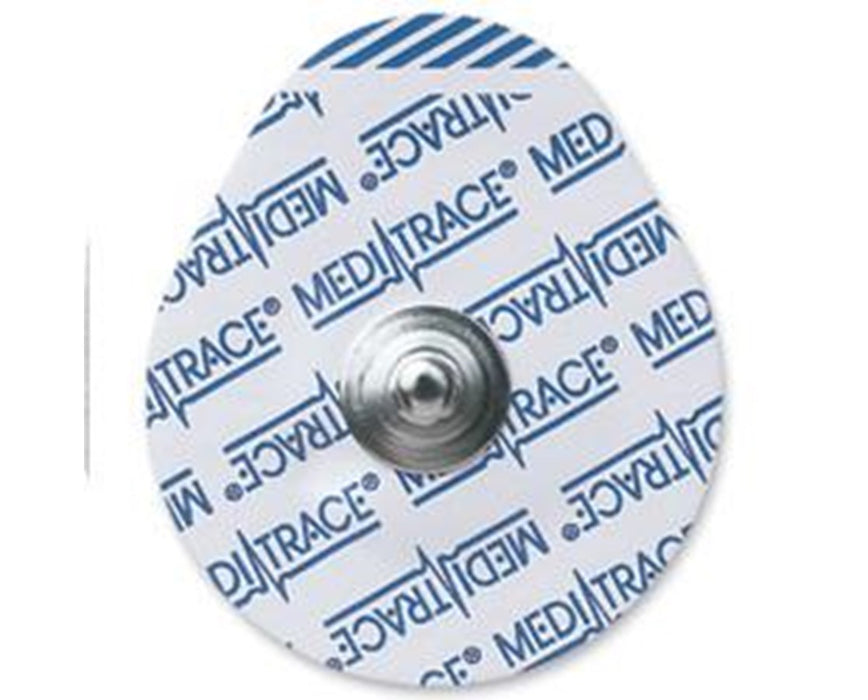
\includegraphics[height=1.5cm,keepaspectratio]{imagenes/electrodo_meditrace.jpg}\\[0.03cm]
                    \tiny \textbf{Meditrace}\\
                    \tiny Ag/AgCl con gel sólido
                \end{column}
                \begin{column}{0.48\linewidth}
                    \centering
                    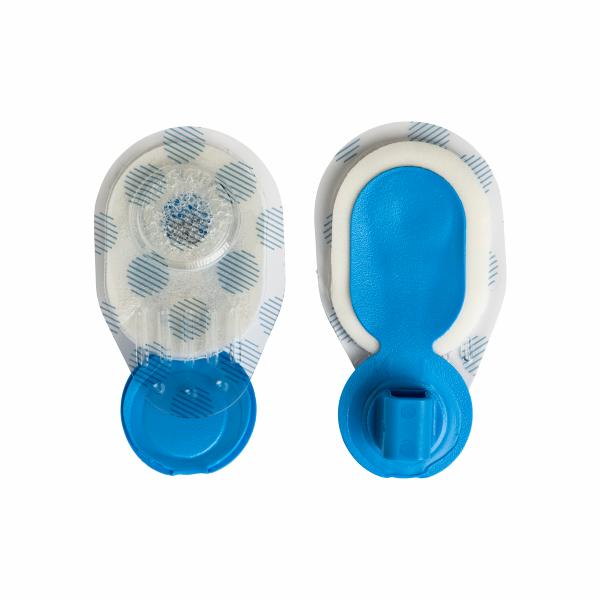
\includegraphics[height=1.5cm,keepaspectratio]{imagenes/electrodo_premium.jpg}\\[0.03cm]
                    \tiny \textbf{Premium}\\
                    \tiny Ag/AgCl wet-gel con broche desfasado
                \end{column}
            \end{columns}
        \end{column}
    \end{columns}
\end{frame}

% ------------------------------------------------------------------------------
% Slide: Electrodos de copa de oro: por qué no sirvieron para hablar
% ------------------------------------------------------------------------------
\begin{frame}{Electrodos reutilizables: copas de oro y descarte \hfill \textnormal{\footnotesize 16/10/2026}}
    \begin{columns}[c]
        \begin{column}{0.50\textwidth}
            \footnotesize
            \begin{block}{Por qué los probamos}
                En EEG se usan copas de oro con pasta conductora para evitar gastar descartables.
            \end{block}
            \vspace{0.03cm}
            \begin{block}{Qué pasó durante las pruebas}
                \begin{itemize}
                    \item \textbf{Se despegan al hablar:} La piel se estira al articular y la pasta no tiene fijación mecánica.
                    \item \textbf{Saturan el AD620 ($G \approx 495\,\text{V/V}$):} Al despegarse a medias se corta el contacto e inyecta picos masivos de 50~Hz.
                \end{itemize}
            \end{block}
            \vspace{0.03cm}
            \begin{block}{Decisión}
                Descarte total para habla. El parche adhesivo (Meditrace) es indispensable para tolerar la tracción facial.
            \end{block}
        \end{column}
        \begin{column}{0.48\textwidth}
            \centering
            \textbf{\footnotesize Comparación de electrodos}\\[0.02cm]
            \begin{columns}[c]
                \begin{column}{0.49\linewidth}
                    \centering
                    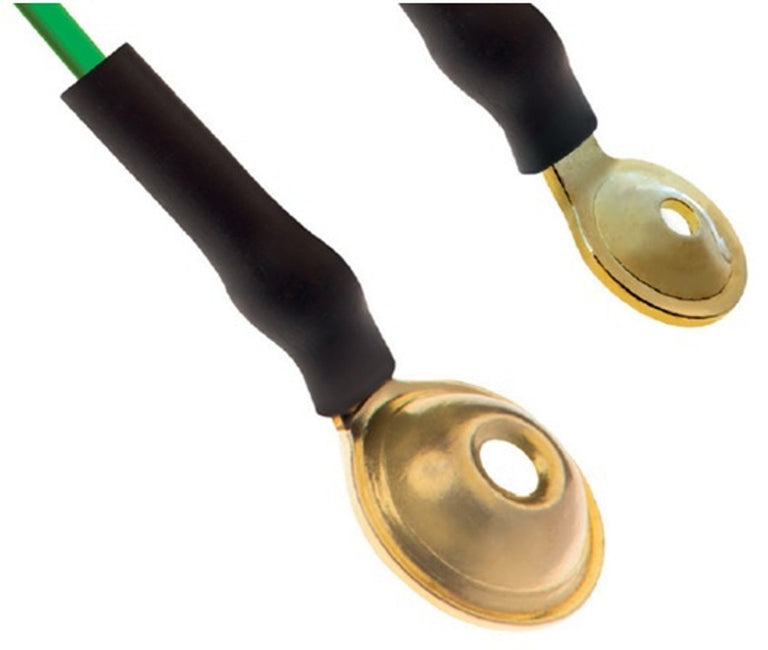
\includegraphics[height=1.3cm,keepaspectratio]{imagenes/electrodo_copa_oro.jpg}\\[0.01cm]
                    \tiny \textbf{Copa de oro}\\
                    \tiny Sin fijación mecánica.\\
                    \tiny Se despega al hablar.
                \end{column}
                \begin{column}{0.49\linewidth}
                    \centering
                    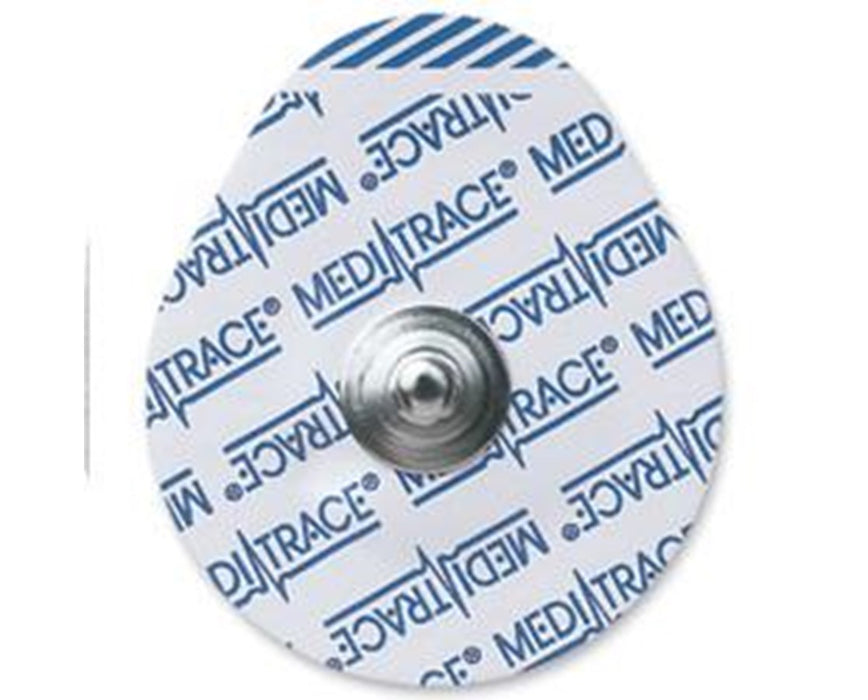
\includegraphics[height=1.3cm,keepaspectratio]{imagenes/electrodo_meditrace.jpg}\\[0.01cm]
                    \tiny \textbf{Meditrace}\\
                    \tiny Parche adhesivo.\\
                    \tiny Tolera la tracción facial.
                \end{column}
            \end{columns}
            \vspace{0.03cm}
            \begin{block}{Comportamiento en registro}
                \scriptsize
                \begin{itemize}
                    \item \textbf{Copa de oro:} Saltos de continua y saturación en 50~Hz.
                    \item \textbf{Meditrace:} Línea de base quieta y contacto firme.
                \end{itemize}
            \end{block}
        \end{column}
    \end{columns}
\end{frame}

% ------------------------------------------------------------------------------
% Slide: Tamaño de pines: grandes vs chicos
% ------------------------------------------------------------------------------
\begin{frame}{Tamaño de pines: electrodos grandes vs chicos \hfill \textnormal{\footnotesize 10/06--16/10/2026}}
    \begin{columns}[c]
        \begin{column}{0.48\textwidth}
            \footnotesize
            \begin{block}{El compromiso entre área censada y selectividad}
                El área metálica del pin cambia cómo ve el músculo y qué tan sensible es a la colocación:
            \end{block}
            \vspace{0.06cm}
            \begin{itemize}
                \item \textbf{Pines grandes:} Abarcan un volumen muscular mayor. Si el electrodo queda 1 o 2~mm corrido respecto a la sesión anterior, la señal casi no cambia. Permite repetir mediciones en distintos días con el mismo mapa de vocales.
                \item \textbf{Pines chicos:} Captan una zona muy puntual. Tienen la selectividad necesaria para separar músculos pegados (como orbicular y mentoniano), pero una pequeña variación milimétrica altera la amplitud.
                \item \textbf{Pines medianos:} No dieron ventaja clara; sufrieron deriva al hablar continuo.
            \end{itemize}
        \end{column}
        \begin{column}{0.50\textwidth}
            \centering
            \includegraphics[width=\textwidth,height=0.82\textheight,keepaspectratio]{imagenes/lucas_pines_grandes_tomas_panel.png}\\[0.05cm]
            \scriptsize Tres días con pines grandes: el mapa se mantiene estable sin corrección por software.
        \end{column}
    \end{columns}
\end{frame}

% ==============================================================================
% SECCIÓN: Exploración Anatómica Facial y Montajes
% ==============================================================================
\section{Exploración Anatómica Facial y Montajes}

% ------------------------------------------------------------------------------
% Slide: Sensores fijos de la cara: mentón y labio superior
% ------------------------------------------------------------------------------
\begin{frame}{Sensores fijos de la cara: mentón y labio superior \hfill \textnormal{\footnotesize 30/08--18/09/2026}}
    \begin{columns}[c]
        \begin{column}{0.48\textwidth}
            \scriptsize
            \begin{block}{Dos canales de referencia en todos los ensayos}
                En las mediciones mantuvimos dos puntos invariables para anclar la articulación:
            \end{block}
            \vspace{0.03cm}
            \begin{itemize}\setlength{\itemsep}{1pt}\setlength{\parskip}{0pt}
                \item \textbf{Canal 0: Mentón - Digástrico anterior}
                \begin{itemize}\setlength{\itemsep}{0pt}\setlength{\parskip}{0pt}
                    \item Mide el descenso de mandíbula al abrir la boca.
                    \item Es la señal dominante de la vocal /a/.
                \end{itemize}
                \item \textbf{Canal 2: Labio superior - Orbicular}
                \begin{itemize}\setlength{\itemsep}{0pt}\setlength{\parskip}{0pt}
                    \item Mide el cierre de labios y la protrusión hacia adelante.
                    \item Detecta las vocales redondas /o/ y /u/.
                \end{itemize}
            \end{itemize}
            \vspace{0.03cm}
            \begin{block}{Qué faltaba resolver}
                Con estos dos canales no se distingue la sonrisa de /e/ e /i/. Hacía falta un tercer sensor en la mejilla para captar la tracción lateral de la boca.
            \end{block}
        \end{column}
        \begin{column}{0.50\textwidth}
            \centering
            \includegraphics[width=\textwidth,height=0.80\textheight,keepaspectratio]{imagenes/candela_canales_fijos.png}
        \end{column}
    \end{columns}
\end{frame}

% ------------------------------------------------------------------------------
% Slide: Exploración de la mejilla: cuatro tríadas en Candela
% ------------------------------------------------------------------------------
\begin{frame}{Exploración de la mejilla: cuatro tríadas en Candela \hfill \textnormal{\footnotesize 30/08--18/09/2026}}
    \begin{columns}[c]
        \begin{column}{0.48\textwidth}
            \centering
            \textbf{\footnotesize Montajes en la mejilla de Candela}\\[0.1cm]
            \includegraphics[width=\textwidth,height=0.74\textheight,keepaspectratio]{imagenes/candela_4_montajes_fotos_2x2.png}
        \end{column}
        \begin{column}{0.50\textwidth}
            \centering
            \textbf{\footnotesize Mapas 2D obtenidos por PCA}\\[0.1cm]
            \includegraphics[width=\textwidth,height=0.74\textheight,keepaspectratio]{imagenes/candela_4_pcas_grid.png}
        \end{column}
    \end{columns}
    \vspace{0.1cm}
    \centering
    \scriptsize
    \textbf{30/08:} Sensor junto a la comisura; separa /o/ de /u/. \quad
    \textbf{01/09:} Cigomático medio; capta la sonrisa de /e/.\\
    \textbf{16/09:} Tracción oblicua alta; aísla nítidamente la /i/. \quad
    \textbf{18/09:} Confluencia labial en modíolo.
\end{frame}

% ------------------------------------------------------------------------------
% Slide: Reemplazo del digástrico por el masetero
% ------------------------------------------------------------------------------
\begin{frame}{Cambio al masetero: fijación y desacople mandibular \hfill \textnormal{\footnotesize 02/10--08/10/2026}}
    \begin{columns}[c]
        \begin{column}{0.48\textwidth}
            \footnotesize
            \begin{block}{Por qué dejamos el digástrico}
                Abajo de la mandíbula los sensores se despegaban por el sudor y el roce con el cuello. En el masetero el parche apoya sobre plano óseo y no se despega en toda la sesión.
            \end{block}
            \vspace{0.05cm}
            \begin{block}{Respuesta muscular en fonación}
                El masetero es el músculo que aprieta la mandíbula. Al combinarlo con el orbicular y el sensor de sonrisa, separa con mucha nitidez las vocales en 3D.
            \end{block}
            \vspace{0.05cm}
            \begin{block}{Aciertos en tomas 1 a 5}
                \begin{itemize}\scriptsize
                    \item \textbf{100\% de acierto en /e/ y en /i/} por el contraste entre sonrisa y mordida.
                    \item \textbf{94\% de acierto en /a/} por la apertura mandibular completa.
                    \item El único solapamiento que quedó fue entre /o/ y /u/ por compartir el cierre labial.
                \end{itemize}
            \end{block}
        \end{column}
        \begin{column}{0.50\textwidth}
            \centering
            \includegraphics[width=\textwidth,height=0.86\textheight,keepaspectratio]{imagenes/masetero_panel_completo.png}
        \end{column}
    \end{columns}
\end{frame}

% ------------------------------------------------------------------------------
% Slide: Dinámica temporal: secuencia de disparo masetero y orbicular
% ------------------------------------------------------------------------------
\begin{frame}{Dinámica temporal: orden de disparo de masetero y labios \hfill \textnormal{\footnotesize 08/10/2026}}
    \begin{columns}[c]
        \begin{column}{0.48\textwidth}
            \footnotesize
            \begin{block}{El retardo de disparo de cada músculo}
                No sólo cuenta cuánta amplitud genera cada músculo, sino en qué momento exacto arranca respecto al audio de la voz:
            \end{block}
            \vspace{0.05cm}
            \begin{itemize}\scriptsize
                \item \textbf{Vocal /a/ - El masetero entra al final:}\\
                Pico a $+118.7$\,ms después de emitir sonido. No abre la boca, sino que frena la mandíbula y la vuelve a cerrar.
                \vspace{0.04cm}
                \item \textbf{Vocal /i/ - Fijación previa de la mordida:}\\
                El masetero dispara $-221.0$\,ms antes del audio trabando la mandíbula, y recién después actúa el labio ($+67.7$\,ms).
                \vspace{0.04cm}
                \item \textbf{Vocal /u/ - Trompita labial anticipada:}\\
                El masetero queda quieto ($2.3\,\mu\text{V}$), mientras el orbicular se anticipa fuertemente ($-239.7$\,ms) para estirar los labios hacia afuera.
            \end{itemize}
        \end{column}
        \begin{column}{0.50\textwidth}
            \centering
            \includegraphics[width=\textwidth,height=0.86\textheight,keepaspectratio]{imagenes/masetero_latencia_secuencia_vertical.png}
        \end{column}
    \end{columns}
\end{frame}

% ------------------------------------------------------------------------------
% Slide: Atlas de activación: especialización de cada músculo
% ------------------------------------------------------------------------------
\begin{frame}{Atlas de activación: especialización de cada músculo \hfill \textnormal{\footnotesize 01/06--18/09/2026}}
    \begin{columns}[c]
        \begin{column}{0.48\textwidth}
            \small
            \begin{block}{Músculos que responden a una sola acción}
                Al promediar repeticiones, cada músculo se encarga casi con exclusividad de ciertos movimientos:
            \end{block}
            \vspace{0.08cm}
            \begin{itemize}\small
                \item \textbf{Cigomático - Sonrisa:}\\
                Dispara temprano y con fuerza ($-229$\,ms) sólo en /i/. En /o/ y /u/ queda totalmente en silencio.
                \vspace{0.05cm}
                \item \textbf{Orbicular - Labios:}\\
                Se activa para apretar o hacer trompita en /o/ y /u/.
                \vspace{0.05cm}
                \item \textbf{Digástrico - Mentón:}\\
                Dispara casi únicamente al abrir la boca para la vocal /a/.
            \end{itemize}
        \end{column}
        \begin{column}{0.50\textwidth}
            \centering
            \includegraphics[width=\textwidth,height=0.78\textheight,keepaspectratio]{imagenes/panel_triada_con_lucas_orbi.png}
        \end{column}
    \end{columns}
\end{frame}

% ------------------------------------------------------------------------------
% Slide: Atlas de activación: consistencia entre distintas personas
% ------------------------------------------------------------------------------
\begin{frame}{Atlas de activación: consistencia inter-sujeto \hfill \textnormal{\footnotesize 01/06--16/09/2026}}
    \begin{columns}[c]
        \begin{column}{0.48\textwidth}
            \small
            \begin{block}{Músculos que hacen lo mismo entre personas}
                Aunque la anatomía y la forma de la cara cambien, los movimientos articulatorios básicos se conservan:
            \end{block}
            \vspace{0.08cm}
            \begin{itemize}\small
                \item \textbf{Vientre anterior y mentón para la /a/:}\\
                Tanto en Lucas (10/07) como en Petra (28/08), abrir la mandíbula activa de forma aislada este canal mientras los otros descansan.
                \vspace{0.05cm}
                \item \textbf{Orbicular para la /o/ y la /u/:}\\
                Tanto en Candela (16/09) como en Lucas (01/06), el cierre labial produce picos gemelos en ambas vocales redondas.
            \end{itemize}
        \end{column}
        \begin{column}{0.50\textwidth}
            \centering
            \includegraphics[width=\textwidth,height=0.74\textheight,keepaspectratio]{imagenes/panel_comparativa_sujetos_final.png}
        \end{column}
    \end{columns}
\end{frame}

% ------------------------------------------------------------------------------
% Slide: Atlas de activación: músculos con respuestas particulares
% ------------------------------------------------------------------------------
\begin{frame}{Atlas de activación: músculos con respuestas particulares \hfill \textnormal{\footnotesize 30/08--18/09/2026}}
    \begin{columns}[c]
        \begin{column}{0.48\textwidth}
            \small
            \begin{block}{Patrones articulatorios secundarios}
                Músculos que mostraron respuestas complementarias:
            \end{block}
            \vspace{0.08cm}
            \begin{itemize}\small
                \item \textbf{Risorio - Tracción lateral:}\\
                Arranca muy temprano en /i/ ($-165$\,ms) y sostiene tensión en /e/ y /a/ por estirar la comisura hacia afuera.
                \vspace{0.05cm}
                \item \textbf{Modíolo - Nodo comisural:}\\
                Cruce de labios y mejilla. Responde con picos anticipados en /o/ ($-150$\,ms), /u/ ($-155$\,ms) e /i/ ($-151$\,ms).
                \vspace{0.05cm}
                \item \textbf{Platisma - Cuello:}\\
                Músculo superficial que se enciende de forma anticipada únicamente en /e/ ($-243$\,ms) e /i/ ($-307$\,ms).
            \end{itemize}
        \end{column}
        \begin{column}{0.50\textwidth}
            \centering
            \includegraphics[width=\textwidth,height=0.78\textheight,keepaspectratio]{imagenes/panel_musculos_particulares_final.png}
        \end{column}
    \end{columns}
\end{frame}

% ==============================================================================
% SECCIÓN: Exploración para Separar O y U
% ==============================================================================
\section{Exploración para Separar O y U}

% ------------------------------------------------------------------------------
% Slide: Exploración para Separar O y U: Vientre Anterior del Digástrico
% ------------------------------------------------------------------------------
\begin{frame}{Separando /o/ de /u/: vientre anterior del digástrico \hfill \textnormal{\footnotesize 14/10/2026}}
    \begin{columns}[c]
        \begin{column}{0.48\textwidth}
            \footnotesize
            \begin{block}{Por qué se probó}
                Pusimos el sensor CH0 en el vientre anterior (cuello) con pines chicos para medir la apertura de mandíbula frente al labio.
            \end{block}
            \vspace{0.04cm}
            \begin{block}{Qué pasó en las pruebas}
                \begin{itemize}
                    \item En 2D insinuó un desvío, pero K-Means mezcló /o/ y /u/ (50\% de confusión).
                    \item Si el electrodo se pegaba cruzado a 90°, la señal caía al piso (macro 44.3\%); exigió alineación longitudinal estricta con las fibras musculares.
                \end{itemize}
            \end{block}
            \vspace{0.04cm}
            \begin{block}{Conclusión}
                \begin{itemize}
                    \item Sirve para resolver la /a/ al abrir la boca, pero no separa el redondeo de /o/ frente al de /u/.
                    \item Esto motivó trasladar el sensor exploratorio hacia el \textbf{mentoniano}.
                \end{itemize}
            \end{block}
        \end{column}
        \begin{column}{0.50\textwidth}
            \centering
            \textbf{\footnotesize Montaje experimental: vientre anterior en cuello}\\[0.01cm]
            \includegraphics[width=\textwidth,height=1.5cm,keepaspectratio]{imagenes/digastrico_foto_cuello.png}\\[0.01cm]
            \tiny \textbf{CH0:} Digástrico (cuello) | \textbf{CH1:} Masetero | \textbf{CH2:} Orbicular\\[0.04cm]
            \textbf{\footnotesize Proyecciones PCA 3D: solapamiento de /o/ y /u/}\\[0.01cm]
            \includegraphics[width=\textwidth,height=1.7cm,keepaspectratio]{imagenes/pca_3d_aciertos_errores_digastrico_inicial.png}\\[0.01cm]
            \tiny \textbf{PC1-PC3 y PC2-PC3:} Las muestras de /o/ y /u/ quedan en el mismo cluster.
        \end{column}
    \end{columns}
\end{frame}

% ------------------------------------------------------------------------------
% Slide: Exploración para Separar O y U: Músculo Mentoniano
% ------------------------------------------------------------------------------
\begin{frame}{Separando /o/ de /u/: músculo mentoniano \hfill \textnormal{\footnotesize 15/10/2026}}
    \begin{columns}[c]
        \begin{column}{0.48\textwidth}
            \footnotesize
            \begin{block}{Por qué se probó}
                Pusimos CH0 en el mentoniano con pines chicos buscando captar el movimiento del labio inferior para despegar /o/ de /u/.
            \end{block}
            \vspace{0.04cm}
            \begin{block}{Arrastre pasivo de la piel}
                \begin{itemize}
                    \item Al articular, la piel del mentón se deforma solidaria con el labio inferior. No es contracción propia, sino tracción mecánica pasiva.
                    \item Probamos \textbf{bajar los sensores 1.5 cm hacia abajo}, pero el arrastre de la piel persistió.
                \end{itemize}
            \end{block}
            \vspace{0.04cm}
            \begin{block}{Resultado en PCA 3D}
                \begin{itemize}
                    \item En 3D apenas asomó un desvío en PC3: /o/ y /u/ quedaron con \textbf{50.0\% de confusión}.
                    \item El mentón no desacopla el redondeo; nos llevó a migrar hacia el \textbf{modíolo}.
                \end{itemize}
            \end{block}
        \end{column}
        \begin{column}{0.50\textwidth}
            \centering
            \textbf{\footnotesize Montaje experimental: músculo mentoniano}\\[0.01cm]
            \includegraphics[width=\textwidth,height=1.5cm,keepaspectratio]{imagenes/mentoniano_foto_frontal.png}\\[0.01cm]
            \tiny \textbf{CH0:} Mentoniano (pines chicos) | \textbf{CH1:} Masetero | \textbf{CH2:} Orbicular\\[0.04cm]
            \textbf{\footnotesize Proyecciones PCA 3D: confusión entre /o/ y /u/}\\[0.01cm]
            \includegraphics[width=\textwidth,height=1.7cm,keepaspectratio]{imagenes/pca_3d_aciertos_errores_mentoniano.png}\\[0.01cm]
            \tiny \textbf{PC1-PC3 y PC2-PC3:} Las muestras de /o/ y /u/ se solapan en el cuadrante inferior.
        \end{column}
    \end{columns}
\end{frame}

% ------------------------------------------------------------------------------
% Slide: Exploración para Separar O y U: El Nodo del Modíolo
% ------------------------------------------------------------------------------
\begin{frame}{Separando /o/ de /u/: el nodo del modíolo \hfill \textnormal{\footnotesize 16/10/2026}}
    \begin{columns}[c]
        \begin{column}{0.48\textwidth}
            \scriptsize
            \begin{block}{El problema mecánico entre /o/ y /u/}
                Ambas vocales comparten el cierre del orbicular, por lo que colapsan en el mismo cluster con montajes comunes.
            \end{block}
            \vspace{0.02cm}
            \begin{block}{El punto anatómico del modíolo}
                \begin{itemize}
                    \item El \textbf{modíolo} es el nodo comisural donde confluyen risorio, orbicular, buccinador y depresores.
                    \item Permite desacoplar el redondeo abierto de /o/ frente a la protrusión cerrada de /u/.
                \end{itemize}
            \end{block}
            \vspace{0.02cm}
            \begin{block}{Resultados en PCA 3D}
                \begin{itemize}
                    \item En 2D quedan contiguas, pero la tercera componente (PC3) las separa con \textbf{82.1\% de acierto}.
                    \item Dio \textbf{71.4\%} en /o/, \textbf{92.9\%} en /u/ y \textbf{84.6\% macro} en las 5 vocales.
                \end{itemize}
            \end{block}
        \end{column}
        \begin{column}{0.50\textwidth}
            \centering
            \textbf{\footnotesize Montaje experimental: modíolo, masetero y orbicular}\\[0.02cm]
            \includegraphics[width=\textwidth,height=1.6cm,keepaspectratio]{imagenes/modiolo_montaje_electrodos_panel.png}\\[0.02cm]
            \tiny \textbf{CH0:} Modíolo (comisura) | \textbf{CH1:} Masetero | \textbf{CH2:} Orbicular\\[0.06cm]
            \textbf{\footnotesize Proyecciones PCA 3D: desacople en PC3}\\[0.02cm]
            \includegraphics[width=\textwidth,height=1.8cm,keepaspectratio]{imagenes/pca_3d_aciertos_errores_modiolo.png}\\[0.02cm]
            \tiny \textbf{PC1-PC3 y PC2-PC3:} Separación efectiva de /o/ (violeta) frente a /u/ (naranja).
        \end{column}
    \end{columns}
\end{frame}

% ==============================================================================
% SECCIÓN: Análisis Previos - Mediciones con Lucas y Petra
% ==============================================================================
\section{Análisis Previos - Mediciones con Lucas y Petra}

% ------------------------------------------------------------------------------
% Slide: Análisis Previos: Estabilidad Inter-Día en Lucas con Pines Grandes
% ------------------------------------------------------------------------------
\begin{frame}{Análisis previos: estabilidad en Lucas con pines grandes \hfill \textnormal{\footnotesize 01/06--10/06/2026}}
    \begin{columns}[c]
        \begin{column}{0.48\textwidth}
            \small
            \begin{block}{Tomas T1 a T7 - Junio 2026}
                Medimos a Lucas en 3 días distintos (01/06, 03/06 y 10/06). Despegando los sensores cada día y volviéndolos a colocar, el mapa de vocales se mantuvo en el mismo lugar sin necesidad de corregir nada por software.
            \end{block}
            \vspace{0.1cm}
            \begin{block}{Efecto del tamaño del pin}
                Los pines grandes abarcan más área muscular: perdonan si el parche se corre uno o dos milímetros. Con pines chicos la señal es más selectiva, pero cualquier desplazamiento mínimo cambia la escala.
            \end{block}
        \end{column}
        \begin{column}{0.50\textwidth}
            \centering
            \includegraphics[width=\textwidth,height=0.82\textheight,keepaspectratio]{imagenes/lucas_pines_grandes_tomas_panel.png}\\[0.05cm]
            \scriptsize PCA en 3 días distintos: la /a/ siempre arriba, sonrisas a la izquierda y /o/-/u/ a la derecha.
        \end{column}
    \end{columns}
\end{frame}

% ------------------------------------------------------------------------------
% Slide: Análisis Previos: Consistencia Anatómica en Petra
% ------------------------------------------------------------------------------
\begin{frame}{Análisis previos: consistencia anatómica en Petra \hfill \textnormal{\footnotesize 21/08--28/08/2026}}
    \begin{columns}[c]
        \begin{column}{0.48\textwidth}
            \small
            \begin{block}{Mediciones del 21/08 y 28/08}
                Probamos en Petra con una semana de diferencia usando vientre anterior en mentón, cigomático y elevador del labio.
            \end{block}
            \vspace{0.1cm}
            \begin{block}{Músculos que conservan su función}
                \begin{itemize}
                    \item Al abrir la boca para la /a/, el mentón se enciende al 100\% y los demás quedan apagados.
                    \item Para /o/ y /u/, el orbicular dispara en bloque mientras el mentón queda en silencio.
                    \item La función motora básica de cada músculo es universal entre Lucas y Petra.
                \end{itemize}
            \end{block}
        \end{column}
        \begin{column}{0.50\textwidth}
            \centering
            \includegraphics[width=\textwidth,height=0.74\textheight,keepaspectratio]{imagenes/panel_comparativa_sujetos_final.png}\\[0.05cm]
            \scriptsize Mismos músculos disparando en las mismas vocales entre Lucas y Petra.
        \end{column}
    \end{columns}
\end{frame}

% ==============================================================================
% SECCIÓN: Análisis de Datos y Modelado
% ==============================================================================
\section{Análisis de Datos y Modelado}

% ------------------------------------------------------------------------------
% Slide: Acondicionamiento por reposo: desacoplando /o/ de /u/
% ------------------------------------------------------------------------------
\begin{frame}{Acondicionamiento por reposo: desacoplando /o/ de /u/ \hfill \textnormal{\footnotesize 18/09--20/09/2026}}
    \begin{columns}[c]
        \begin{column}{0.50\textwidth}
            \small
            \begin{block}{Deriva de la línea de base entre sesiones}
                \footnotesize El contacto del gel con la piel y la transpiración varían entre sesiones, desplazando el reposo y la escala de cada sensor.
            \end{block}
            \vspace{0.06cm}
            \textbf{\footnotesize Corrección por reposo y rango dinámico:}
            \begin{itemize}
                \scriptsize
                \item Tras el Supremo Tricanal ($M_{\text{supremo}}$), se ajusta canal por canal:
                \vspace{-0.12cm}
                $$\tilde{x}_c(t) = \frac{x_c(t) - \mu_{\text{reposo}, c}}{P_{95}(x_c) - \mu_{\text{reposo}, c}}$$
                \vspace{-0.12cm}
                \item $\mu_{\text{reposo}}$: Línea de base en reposo antes de la fonación.
                \item $P_{95}$: Rango dinámico útil de contracción (percentil 95).
            \end{itemize}
            \vspace{0.05cm}
            \begin{block}{Desacople entre /o/ y /u/}
                \scriptsize La confusión entre /o/ y /u/ no era muscular, sino un corrimiento del reposo del labio. Al restarlo, los dos grupos se separan en el mapa (LDA 86.8\%).
            \end{block}
        \end{column}
        \begin{column}{0.48\textwidth}
            \centering
            \textbf{\footnotesize Comparativa en el mapa 2D de Lucas}\\[0.1cm]
            \includegraphics[width=\textwidth,height=0.68\textheight,keepaspectratio]{imagenes/lucas_pca_sin_vs_con_reposo_comparativa.png}\\[0.1cm]
            \scriptsize
            \textbf{Izquierda - Sin reposo:} /o/ y /u/ solapadas.\\
            \textbf{Derecha - Con reposo:} Grupos fonéticos separados (LDA 86.8\%).
        \end{column}
    \end{columns}
\end{frame}

% ------------------------------------------------------------------------------
% Slide: Autoencoder convolucional ortogonal - 88% no supervisado
% ------------------------------------------------------------------------------
\begin{frame}{Autoencoder convolucional ortogonal: récord del 88\% \hfill \textnormal{\footnotesize 22/09/2026}}
    \begin{columns}[c]
        \begin{column}{0.48\textwidth}
            \small
            \begin{block}{Por qué fallaba el autoencoder común}
                Entrenado sólo con pérdida MSE, amontona las representaciones porque nada le exige usar dimensiones independientes del espacio latente.
            \end{block}
            \vspace{0.05cm}
            \textbf{\footnotesize Autoencoder convolucional ortogonal:}
            \begin{itemize}
                \scriptsize
                \item \textbf{Cero etiquetas en el entrenamiento:} Aprende a reconstruir la señal sin supervisión.
                \item Regularización ortogonal en los pesos y decorrelación latente.
                \item \textbf{Récord en Lucas:} \textbf{88\% con GMM no supervisado} (evaluado a ciegas con K-Means/GMM y asignación húngara, sin usar etiquetas al entrenar).
                \item \textbf{Mapa canónico en cruz:}
                \begin{itemize}
                    \scriptsize
                    \item Arriba (+Y): Apertura bucal (/a/).
                    \item Eje vertical: Sonrisas (/i/, /e/).
                    \item Izquierda (-X): Cierre de labios (/o/, /u/).
                \end{itemize}
            \end{itemize}
        \end{column}
        \begin{column}{0.50\textwidth}
            \centering
            \textbf{\footnotesize Autoencoder estándar vs ortogonal}\\[0.08cm]
            \includegraphics[width=\textwidth,height=0.70\textheight,keepaspectratio]{imagenes/lucas_ae_comun_vs_ortogonal_comparativa.png}\\[0.08cm]
            \scriptsize
            \textbf{Izquierda:} El autoencoder estándar mezcla fonemas.\\
            \textbf{Derecha:} La red ortogonal abre la cruz (88\% GMM no supervisado / LDA).
        \end{column}
    \end{columns}
\end{frame}

% ------------------------------------------------------------------------------
% Slide: Habla continua: decodificación al vuelo con gate doble en P5
% ------------------------------------------------------------------------------
\begin{frame}{Habla continua: decodificación con gate doble en P5 \hfill \textnormal{\footnotesize 24/09/2026}}
    \begin{columns}[c]
        \begin{column}{0.48\textwidth}
            \small
            \begin{block}{Prueba en grabación continua P5}
                Evaluamos una secuencia continua de 123 fonaciones seguidas (A-E-I-O-U) que la red nunca vio en el entrenamiento.
            \end{block}
            \vspace{0.1cm}
            \textbf{Detección y segmentación temporal:}
            \begin{itemize}
                \item \textbf{Algoritmo de gate doble:} Dos umbrales de energía para marcar con precisión el inicio y el final de cada pulso.
                \item \textbf{Ajuste del retardo electromecánico:} El músculo se enciende unos 350~ms antes del sonido en el micrófono; sincronizamos esa ventana.
                \item \textbf{Resultado:} \textbf{82.9\% de acierto} (102 de 123 vocales decodificadas al vuelo) sin reentrenar la red.
            \end{itemize}
        \end{column}
        \begin{column}{0.50\textwidth}
            \centering
            \includegraphics[width=\textwidth,height=0.82\textheight,keepaspectratio]{imagenes/comparativa_gate_doble_primeros_pulsos.png}
        \end{column}
    \end{columns}
\end{frame}

% ------------------------------------------------------------------------------
% Slide: Transferencia inter-sujeto: rotación y simetría en el espacio latente
% ------------------------------------------------------------------------------
\begin{frame}{Transferencia inter-sujeto: rotación en el espacio latente \hfill \textnormal{\footnotesize 26/09--28/09/2026}}
    \begin{columns}[c]
        \begin{column}{0.48\textwidth}
            \small
            \begin{block}{El mapa motor aparece rotado}
                Al evaluar a otro participante (Santi, Petra, Candela) o volver a pegar sensores otro día, el mapa interno aparece girado en el plano.
            \end{block}
            \vspace{0.1cm}
            \textbf{Por qué cae la red si no calibramos:}
            \begin{itemize}
                \item En Candela el mapa aparece girado unos $-95^\circ$ por la orientación en que se pegaron los electrodos.
                \item Las fronteras de decisión fijadas con Lucas ya no coinciden y el acierto cae por debajo del 68\%.
                \item Cada persona conserva sus clusters formados, pero están desalineados en el espacio.
            \end{itemize}
        \end{column}
        \begin{column}{0.50\textwidth}
            \centering
            \includegraphics[width=\textwidth,height=0.82\textheight,keepaspectratio]{imagenes/panel_candela_3_configuraciones_nativas.png}
        \end{column}
    \end{columns}
\end{frame}

% ------------------------------------------------------------------------------
% Slide: Arquitectura del sistema: esquema de decodificación
% ------------------------------------------------------------------------------
\begin{frame}{Arquitectura del sistema: esquema de decodificación \hfill \textnormal{\footnotesize 01/10/2026}}
    \vspace{-0.15cm}
    \begin{center}
    \begin{tikzpicture}[
        every node/.style={font=\sffamily},
        card/.style={
            rectangle, rounded corners=6pt, line width=0.9pt,
            text width=4.35cm, minimum height=2.85cm,
            align=left, inner sep=6pt, anchor=north
        },
        cardbottom/.style={
            rectangle, rounded corners=6pt, line width=1pt,
            text width=14.4cm, minimum height=2.3cm,
            align=left, inner sep=7pt, anchor=north
        },
        carrow/.style={
            -{Stealth[length=3mm, width=2.2mm]}, line width=1.5pt, draw=DarkBlue!75
        }
    ]
        % Fila superior: Las 3 etapas de procesamiento y calibración
        \node[card, draw=Stage1!80!black, fill=Stage1!8] (c1) at (0,0) {
            \colorbox{Stage1}{\textcolor{white}{\textbf{\footnotesize 1. Modelo Base - Lucas}}}\\[0.18cm]
            \scriptsize
            \textbullet~\textbf{Autoencoder 1D:} No supervisado.\\
            \textbullet~\textbf{Variedad canónica:} Mapa 2D de alta cohesión (88--89\%).\\
            \textbullet~\textbf{Pesos congelados:} Red fija en memoria.
        };

        \node[card, draw=Stage2!80!black, fill=Stage2!8] (c2) at (5.05,0) {
            \colorbox{Stage2}{\textcolor{white}{\textbf{\footnotesize 2. Nuevo Usuario}}}\\[0.18cm]
            \scriptsize
            \textbullet~\textbf{Sujeto no visto:} Santi, Petra o Candela.\\
            \textbullet~\textbf{Paso directo:} Inferencia con encoder congelado.\\
            \textbullet~\textbf{Rotación observada:} Mapa rotado ($\sim\!-95^\circ$) por postura de sensores.
        };

        \node[card, draw=Stage3!80!black, fill=Stage3!8] (c3) at (10.1,0) {
            \colorbox{Stage3}{\textcolor{white}{\textbf{\footnotesize 3. Calibración Sara Solla}}}\\[0.18cm]
            \scriptsize
            \textbullet~\textbf{Protocolo rápido:} $<$20 segundos con 3 anclas: /a/, /i/, /u/.\\
            \textbullet~\textbf{Procrustes ortogonal:} Calcula la rotación $O(2)$ al vuelo.\\
            \textbullet~\textbf{Cero reentrenamiento:} Alinea el mapa preservando distancias.
        };

        % Conexiones superiores
        \draw[carrow] (c1.east |- 0,-1.4) -- (c2.west |- 0,-1.4);
        \draw[carrow] (c2.east |- 0,-1.4) -- (c3.west |- 0,-1.4);

        % Fila inferior: Decodificación y fronteras fijas
        \node[cardbottom, draw=Stage4!80!black, fill=Stage4!7] (c4) at (5.05,-3.35) {
            \colorbox{Stage4}{\textcolor{white}{\textbf{\footnotesize 4. Decodificación en tiempo real sobre fronteras fijas}}}\\[0.15cm]
            \begin{minipage}[t]{0.485\textwidth}
                \scriptsize
                \textbullet~\textbf{Fronteras fijas:} El mapa rotado se evalúa sobre las regiones LDA de Lucas.\\
                \textbullet~\textbf{Baja latencia:} $<0.35\text{ ms}$ por fonación, apto para streaming en vivo.
            \end{minipage}\hfill
            \begin{minipage}[t]{0.485\textwidth}
                \scriptsize
                \textbullet~\textbf{83.6\% de acierto global:} 1028 fonaciones reales en 4 sujetos.\\
                \textbullet~\textbf{82.9\% en habla continua:} 102 de 123 fonaciones al vuelo en la secuencia P5.
            \end{minipage}
        };

        % Flecha hacia la fila inferior
        \draw[carrow, draw=Stage3!90!black] (c3.south) -- node[right, font=\tiny\bfseries, text=Stage3!90!black, xshift=2pt] {Proyección alineada} (c4.north -| c3.south);

    \end{tikzpicture}
    \end{center}
\end{frame}

% ------------------------------------------------------------------------------
% Slide: Calibración por rotación: alineación Sara Solla con A-I-U
% ------------------------------------------------------------------------------
\begin{frame}{Calibración por rotación: alineación Sara Solla con A-I-U \hfill \textnormal{\footnotesize 03/10/2026}}
    \begin{columns}[c]
        \begin{column}{0.48\textwidth}
            \small
            \begin{block}{Variedad motora universal}
                La hipótesis de Sara Solla plantea que los comandos articulatorios comparten la misma estructura geométrica en todas las personas, pero los sensores proyectan la señal rotada.
            \end{block}
            \vspace{0.1cm}
            \textbf{Calibración con tres anclas extremas (/a/, /i/, /u/):}
            \begin{itemize}
                \item Las vocales intermedias (/e/, /o/) tienen mayor dispersión y meten ruido al estimar el giro.
                \item Alineando únicamente con los tres vértices articulatorios, la rotación $O(2)$ es exacta e instantánea.
                \item \textbf{1028 fonaciones reales (4 sujetos):} El acierto sube de 68.5\% a \textbf{83.6\%} (Lucas 88\%, Santi 88\%, Petra 78\%, Candela 75\%) sin tocar los pesos de la red.
            \end{itemize}
        \end{column}
        \begin{column}{0.50\textwidth}
            \centering
            \includegraphics[width=\textwidth,height=0.82\textheight,keepaspectratio]{imagenes/figura_paper_variedad_universal_cuatrisujeto.png}
        \end{column}
    \end{columns}
\end{frame}

% ------------------------------------------------------------------------------
% Slide: Conclusiones y próximos pasos
% ------------------------------------------------------------------------------
\begin{frame}{Conclusiones y próximos pasos \hfill \textnormal{\footnotesize Octubre 2026}}
    \begin{columns}[t]
        \begin{column}{0.48\textwidth}
            \small
            \begin{block}{Lo que quedó funcionando}
                \begin{itemize}
                    \item \textbf{Hardware:} Cables mallados bajan el piso de ruido 4 veces sin notch.
                    \item \textbf{Reposo:} Corregir el reposo basal desacopla /o/ de /u/.
                    \item \textbf{Modelo 88\%:} Autoencoder ortogonal aprende sin etiquetas.
                    \item \textbf{Habla continua:} Gate doble decodifica en tiempo real (83\% en P5).
                    \item \textbf{Generalización:} Calibrando con A-I-U alcanza 83.6\% en 4 personas.
                \end{itemize}
            \end{block}
        \end{column}
        \begin{column}{0.48\textwidth}
            \small
            \begin{block}{Próximos pasos de laboratorio}
                \begin{enumerate}
                    \item \textbf{Calibración en la interfaz:} Botón para calibrar la rotación con A-I-U ($<20\,\text{s}$).
                    \item \textbf{Cables mallados en habla continua:} Grabar secuencias largas con blindaje nuevo.
                    \item \textbf{Pines chicos en comisura:} Consolidar el modíolo para cerrar el par /o/ vs /u/.
                    \item \textbf{Cierre del manuscrito:} Integrar el panel cuatrisujeto al reporte final.
                \end{enumerate}
            \end{block}
        \end{column}
    \end{columns}
\end{frame}

\end{document}
